% Created by tikzDevice version 0.10.1 on 2016-12-20 22:02:45
% !TEX encoding = UTF-8 Unicode
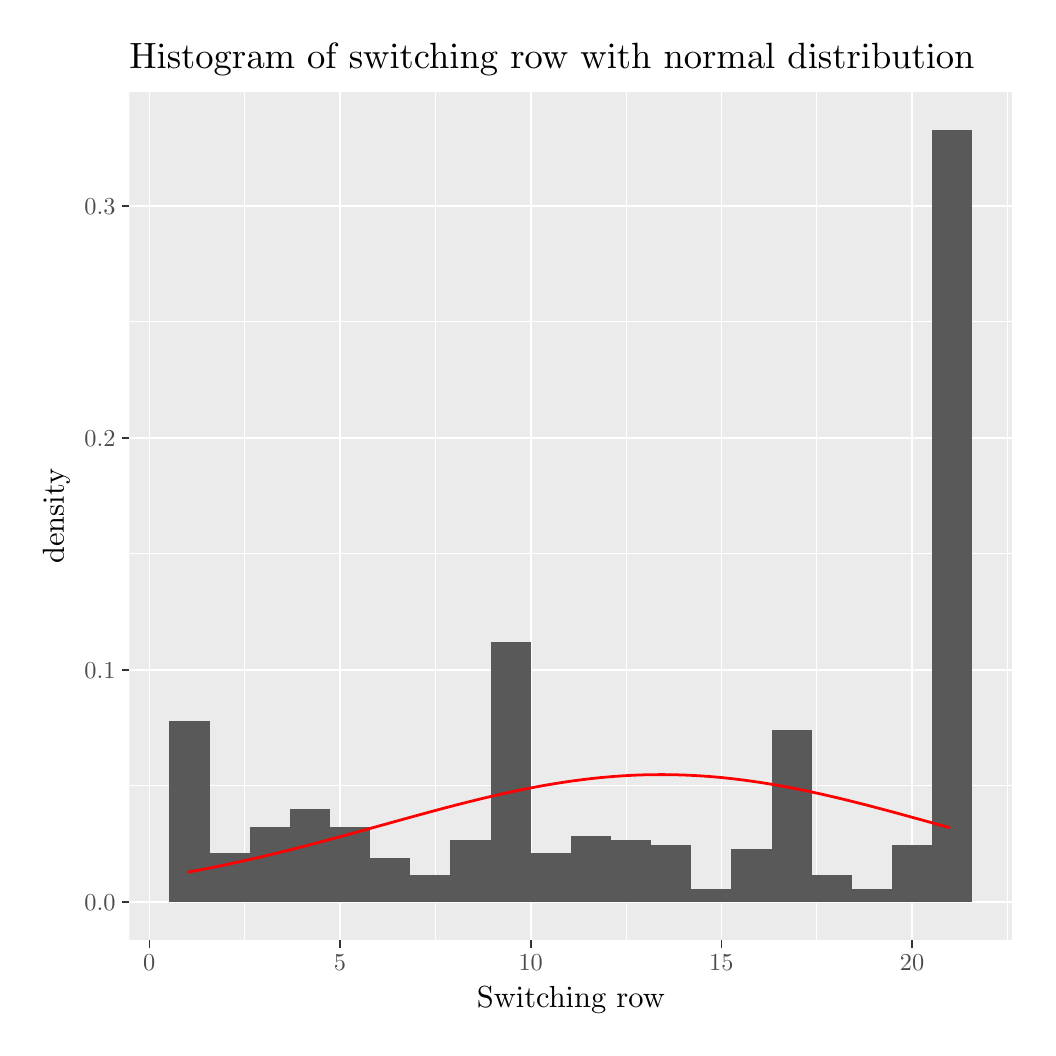
\begin{tikzpicture}[x=1pt,y=1pt]
\definecolor{fillColor}{RGB}{255,255,255}
\path[use as bounding box,fill=fillColor,fill opacity=0.00] (0,0) rectangle (361.35,361.35);
\begin{scope}
\path[clip] (  0.00,  0.00) rectangle (361.35,361.35);
\definecolor{drawColor}{RGB}{255,255,255}
\definecolor{fillColor}{RGB}{255,255,255}

\path[draw=drawColor,line width= 0.6pt,line join=round,line cap=round,fill=fillColor] (  0.00,  0.00) rectangle (361.35,361.35);
\end{scope}
\begin{scope}
\path[clip] ( 36.71, 31.53) rectangle (355.85,338.21);
\definecolor{fillColor}{gray}{0.92}

\path[fill=fillColor] ( 36.71, 31.53) rectangle (355.85,338.21);
\definecolor{drawColor}{RGB}{255,255,255}

\path[draw=drawColor,line width= 0.3pt,line join=round] ( 36.71, 87.40) --
	(355.85, 87.40);

\path[draw=drawColor,line width= 0.3pt,line join=round] ( 36.71,171.25) --
	(355.85,171.25);

\path[draw=drawColor,line width= 0.3pt,line join=round] ( 36.71,255.10) --
	(355.85,255.10);

\path[draw=drawColor,line width= 0.3pt,line join=round] ( 78.42, 31.53) --
	( 78.42,338.21);

\path[draw=drawColor,line width= 0.3pt,line join=round] (147.32, 31.53) --
	(147.32,338.21);

\path[draw=drawColor,line width= 0.3pt,line join=round] (216.23, 31.53) --
	(216.23,338.21);

\path[draw=drawColor,line width= 0.3pt,line join=round] (285.13, 31.53) --
	(285.13,338.21);

\path[draw=drawColor,line width= 0.3pt,line join=round] (354.04, 31.53) --
	(354.04,338.21);

\path[draw=drawColor,line width= 0.6pt,line join=round] ( 36.71, 45.47) --
	(355.85, 45.47);

\path[draw=drawColor,line width= 0.6pt,line join=round] ( 36.71,129.32) --
	(355.85,129.32);

\path[draw=drawColor,line width= 0.6pt,line join=round] ( 36.71,213.17) --
	(355.85,213.17);

\path[draw=drawColor,line width= 0.6pt,line join=round] ( 36.71,297.02) --
	(355.85,297.02);

\path[draw=drawColor,line width= 0.6pt,line join=round] ( 43.96, 31.53) --
	( 43.96,338.21);

\path[draw=drawColor,line width= 0.6pt,line join=round] (112.87, 31.53) --
	(112.87,338.21);

\path[draw=drawColor,line width= 0.6pt,line join=round] (181.77, 31.53) --
	(181.77,338.21);

\path[draw=drawColor,line width= 0.6pt,line join=round] (250.68, 31.53) --
	(250.68,338.21);

\path[draw=drawColor,line width= 0.6pt,line join=round] (319.58, 31.53) --
	(319.58,338.21);
\definecolor{fillColor}{gray}{0.35}

\path[fill=fillColor] ( 51.22, 45.47) rectangle ( 65.72,110.79);

\path[fill=fillColor] ( 65.72, 45.47) rectangle ( 80.23, 63.00);

\path[fill=fillColor] ( 80.23, 45.47) rectangle ( 94.74, 72.55);

\path[fill=fillColor] ( 94.74, 45.47) rectangle (109.24, 78.93);

\path[fill=fillColor] (109.24, 45.47) rectangle (123.75, 72.55);

\path[fill=fillColor] (123.75, 45.47) rectangle (138.26, 61.40);

\path[fill=fillColor] (138.26, 45.47) rectangle (152.76, 55.03);

\path[fill=fillColor] (152.76, 45.47) rectangle (167.27, 67.78);

\path[fill=fillColor] (167.27, 45.47) rectangle (181.77,139.47);

\path[fill=fillColor] (181.77, 45.47) rectangle (196.28, 63.00);

\path[fill=fillColor] (196.28, 45.47) rectangle (210.79, 69.37);

\path[fill=fillColor] (210.79, 45.47) rectangle (225.29, 67.78);

\path[fill=fillColor] (225.29, 45.47) rectangle (239.80, 66.18);

\path[fill=fillColor] (239.80, 45.47) rectangle (254.31, 50.25);

\path[fill=fillColor] (254.31, 45.47) rectangle (268.81, 64.59);

\path[fill=fillColor] (268.81, 45.47) rectangle (283.32,107.60);

\path[fill=fillColor] (283.32, 45.47) rectangle (297.82, 55.03);

\path[fill=fillColor] (297.82, 45.47) rectangle (312.33, 50.25);

\path[fill=fillColor] (312.33, 45.47) rectangle (326.84, 66.18);

\path[fill=fillColor] (326.84, 45.47) rectangle (341.34,324.27);
\definecolor{drawColor}{RGB}{255,0,0}

\path[draw=drawColor,line width= 1.0pt,line join=round] ( 57.75, 56.18) --
	( 60.50, 56.69) --
	( 63.26, 57.21) --
	( 66.01, 57.75) --
	( 68.77, 58.31) --
	( 71.53, 58.88) --
	( 74.28, 59.47) --
	( 77.04, 60.07) --
	( 79.80, 60.68) --
	( 82.55, 61.31) --
	( 85.31, 61.95) --
	( 88.06, 62.61) --
	( 90.82, 63.28) --
	( 93.58, 63.96) --
	( 96.33, 64.65) --
	( 99.09, 65.35) --
	(101.84, 66.06) --
	(104.60, 66.79) --
	(107.36, 67.52) --
	(110.11, 68.25) --
	(112.87, 69.00) --
	(115.63, 69.75) --
	(118.38, 70.51) --
	(121.14, 71.27) --
	(123.89, 72.03) --
	(126.65, 72.80) --
	(129.41, 73.56) --
	(132.16, 74.33) --
	(134.92, 75.09) --
	(137.68, 75.86) --
	(140.43, 76.61) --
	(143.19, 77.37) --
	(145.94, 78.11) --
	(148.70, 78.85) --
	(151.46, 79.58) --
	(154.21, 80.30) --
	(156.97, 81.01) --
	(159.73, 81.70) --
	(162.48, 82.38) --
	(165.24, 83.04) --
	(167.99, 83.69) --
	(170.75, 84.32) --
	(173.51, 84.93) --
	(176.26, 85.52) --
	(179.02, 86.09) --
	(181.77, 86.63) --
	(184.53, 87.15) --
	(187.29, 87.65) --
	(190.04, 88.11) --
	(192.80, 88.55) --
	(195.56, 88.97) --
	(198.31, 89.35) --
	(201.07, 89.70) --
	(203.82, 90.02) --
	(206.58, 90.32) --
	(209.34, 90.57) --
	(212.09, 90.80) --
	(214.85, 90.99) --
	(217.61, 91.15) --
	(220.36, 91.28) --
	(223.12, 91.37) --
	(225.87, 91.42) --
	(228.63, 91.44) --
	(231.39, 91.43) --
	(234.14, 91.38) --
	(236.90, 91.30) --
	(239.65, 91.18) --
	(242.41, 91.03) --
	(245.17, 90.85) --
	(247.92, 90.63) --
	(250.68, 90.38) --
	(253.44, 90.09) --
	(256.19, 89.78) --
	(258.95, 89.43) --
	(261.70, 89.05) --
	(264.46, 88.65) --
	(267.22, 88.21) --
	(269.97, 87.75) --
	(272.73, 87.26) --
	(275.49, 86.75) --
	(278.24, 86.21) --
	(281.00, 85.65) --
	(283.75, 85.06) --
	(286.51, 84.46) --
	(289.27, 83.83) --
	(292.02, 83.19) --
	(294.78, 82.53) --
	(297.53, 81.85) --
	(300.29, 81.16) --
	(303.05, 80.46) --
	(305.80, 79.74) --
	(308.56, 79.01) --
	(311.32, 78.28) --
	(314.07, 77.53) --
	(316.83, 76.78) --
	(319.58, 76.02) --
	(322.34, 75.26) --
	(325.10, 74.50) --
	(327.85, 73.73) --
	(330.61, 72.97) --
	(333.37, 72.20);
\end{scope}
\begin{scope}
\path[clip] (  0.00,  0.00) rectangle (361.35,361.35);
\definecolor{drawColor}{gray}{0.30}

\node[text=drawColor,anchor=base east,inner sep=0pt, outer sep=0pt, scale=  0.88] at ( 31.76, 42.44) {0.0};

\node[text=drawColor,anchor=base east,inner sep=0pt, outer sep=0pt, scale=  0.88] at ( 31.76,126.29) {0.1};

\node[text=drawColor,anchor=base east,inner sep=0pt, outer sep=0pt, scale=  0.88] at ( 31.76,210.14) {0.2};

\node[text=drawColor,anchor=base east,inner sep=0pt, outer sep=0pt, scale=  0.88] at ( 31.76,293.99) {0.3};
\end{scope}
\begin{scope}
\path[clip] (  0.00,  0.00) rectangle (361.35,361.35);
\definecolor{drawColor}{gray}{0.20}

\path[draw=drawColor,line width= 0.6pt,line join=round] ( 33.96, 45.47) --
	( 36.71, 45.47);

\path[draw=drawColor,line width= 0.6pt,line join=round] ( 33.96,129.32) --
	( 36.71,129.32);

\path[draw=drawColor,line width= 0.6pt,line join=round] ( 33.96,213.17) --
	( 36.71,213.17);

\path[draw=drawColor,line width= 0.6pt,line join=round] ( 33.96,297.02) --
	( 36.71,297.02);
\end{scope}
\begin{scope}
\path[clip] (  0.00,  0.00) rectangle (361.35,361.35);
\definecolor{drawColor}{gray}{0.20}

\path[draw=drawColor,line width= 0.6pt,line join=round] ( 43.96, 28.78) --
	( 43.96, 31.53);

\path[draw=drawColor,line width= 0.6pt,line join=round] (112.87, 28.78) --
	(112.87, 31.53);

\path[draw=drawColor,line width= 0.6pt,line join=round] (181.77, 28.78) --
	(181.77, 31.53);

\path[draw=drawColor,line width= 0.6pt,line join=round] (250.68, 28.78) --
	(250.68, 31.53);

\path[draw=drawColor,line width= 0.6pt,line join=round] (319.58, 28.78) --
	(319.58, 31.53);
\end{scope}
\begin{scope}
\path[clip] (  0.00,  0.00) rectangle (361.35,361.35);
\definecolor{drawColor}{gray}{0.30}

\node[text=drawColor,anchor=base,inner sep=0pt, outer sep=0pt, scale=  0.88] at ( 43.96, 20.52) {0};

\node[text=drawColor,anchor=base,inner sep=0pt, outer sep=0pt, scale=  0.88] at (112.87, 20.52) {5};

\node[text=drawColor,anchor=base,inner sep=0pt, outer sep=0pt, scale=  0.88] at (181.77, 20.52) {10};

\node[text=drawColor,anchor=base,inner sep=0pt, outer sep=0pt, scale=  0.88] at (250.68, 20.52) {15};

\node[text=drawColor,anchor=base,inner sep=0pt, outer sep=0pt, scale=  0.88] at (319.58, 20.52) {20};
\end{scope}
\begin{scope}
\path[clip] (  0.00,  0.00) rectangle (361.35,361.35);
\definecolor{drawColor}{RGB}{0,0,0}

\node[text=drawColor,anchor=base,inner sep=0pt, outer sep=0pt, scale=  1.10] at (196.28,  7.44) {Switching row};
\end{scope}
\begin{scope}
\path[clip] (  0.00,  0.00) rectangle (361.35,361.35);
\definecolor{drawColor}{RGB}{0,0,0}

\node[text=drawColor,rotate= 90.00,anchor=base,inner sep=0pt, outer sep=0pt, scale=  1.10] at ( 13.08,184.87) {density};
\end{scope}
\begin{scope}
\path[clip] (  0.00,  0.00) rectangle (361.35,361.35);
\definecolor{drawColor}{RGB}{0,0,0}

\node[text=drawColor,anchor=base west,inner sep=0pt, outer sep=0pt, scale=  1.32] at ( 36.71,346.76) {Histogram of switching row with normal distribution};
\end{scope}
\end{tikzpicture}
